\documentclass[14pt, a4paper, reqno, oneside]{book}
\usepackage{amssymb,latexsym,amscd,amsmath,amsfonts,enumerate,supertabular,enumitem,fancyhdr}
\usepackage{amsmath,amsxtra,amssymb,latexsym, amscd,amsthm}

\usepackage{subfigure}
\usepackage{titlesec}
\usepackage[usehighlevels]{alnumsec}
\usepackage{indentfirst}
\usepackage[utf8]{vietnam}
%\usepackage{amsmath}
\usepackage{graphics}
\usepackage{graphicx}
\usepackage{tabularx}
\usepackage{epic, eepic}
\usepackage{lineno}
\usepackage{array}
\usepackage[mathscr]{eucal}
%\usepackage{amsfonts}
\usepackage[unicode]{hyperref}
\usepackage{titledot}
\usepackage[top=3cm, bottom=3cm, left=3.5cm, right=2cm] {geometry}
\usepackage{eso-pic,calc}
\usepackage{makeidx}
\usepackage{float}
\usepackage{mathptmx}
\listfiles
\titlename{Chương}
%\swapnumbers
\usepackage{listings}
\usepackage{color} % tô màu cho cod
\definecolor{dkgreen}{rgb}{0,0.6,0}
\definecolor{gray}{rgb}{0.5,0.5,0.5}
\definecolor{mauve}{rgb}{0.58,0,0.82}
\lstset{frame=tb,
	language=Python,
	aboveskip=3mm,
	belowskip=3mm,
	showstringspaces=false,
	columns=flexible,
	basicstyle={\small\ttfamily},
	numbers=none,
	numberstyle=\tiny\color{gray},
	keywordstyle=\color{blue},
	commentstyle=\color{dkgreen},
	stringstyle=\color{mauve},
	breaklines=true,
	breakatwhitespace=true,
	tabsize=3
}
\newtheorem{prof}{}
\newtheorem {theorem}{Định lý}[section]
\newtheorem {corollary}[theorem]{Hệ quả}
\newtheorem {lemma}[theorem]{Bổ đề}
\newtheorem {proposition}[theorem]{Mệnh đề}
\newtheorem {definition}[theorem]{Định nghĩa}
\newtheorem{tc}[theorem]{Tiêu chuẩn}
\newtheorem*{main}{Mệnh đề}
\theoremstyle {definition}
\newtheorem {remark}[theorem]{Chú ý}
\newtheorem {example}[theorem]{Ví dụ}
\newtheorem {notation}[theorem]{Kí hiệu}
\newtheorem {note}[theorem]{Nhận xét}
\renewcommand{\proofname}{\textbf{\textit{Chứng minh}}}
\renewcommand{\bibname}{TÀI LIỆU THAM KHẢO}
\renewcommand{\chaptername}{CHƯƠNG}
\renewcommand{\thechapter}{\arabic{chapter}}
\renewcommand{\thesection}{\thechapter.\arabic{section}}
\renewcommand{\thesubsection}{\thesection.\arabic{subsection}}
\renewcommand{\contentsname}{\hspace{100pt}MỤC LỤC}
\newenvironment{example1}[1][Ví dụ 1]{\begin{trivlist}
		\item[\hskip \labelsep {\bfseries #1}]}{\end{trivlist}}
\newenvironment{example2}[1][Ví dụ 2]{\begin{trivlist}
		\item[\hskip \labelsep {\bfseries #1}]}{\end{trivlist}}
\newenvironment{example3}[1][Ví dụ 3]{\begin{trivlist}
		\item[\hskip \labelsep {\bfseries #1}]}{\end{trivlist}}
\newcommand{\dn}[1]{\frac{\partial #1}{\partial \nu }}

\titleformat{\section}
{\normalfont\bfseries}{\thesection.}{1em}{\fontsize 16}{}
\titleformat{\subsection}
{\normalfont\itshape}{\thesubsection.}{1em}{\fontsize 16}{}
\titleformat{\subsubsection}
{\normalfont\bfseries}{\thesubsubsection.}{1em}{\fontsize 14}{}

\def\ba{\mathbf{a}}
\def\bb{\mathbf{b}}
\def\bd{\mathbf{d}}
\def\be{\mathbf{e}}
\def\bm{\mathbf{m}}
\def\bK{\mathbf{K}}
\def\bk{\mathbf{k}}
\def\bM{\mathbf{M}}
\def\bp{\mathbf{p}}
\def\bq{\mathbf{q}}
\def\bx{\mathbf{x}}
\def\by{\mathbf{y}}
\def\bz{\mathbf{z}}
\def\bu{\mathbf{u}}
\def\bv{\mathbf{v}}
\def\bw{\mathbf{w}}

\def\bbx{\bar{\mathbf{x}}}
\def\bbX{\bar{\mathbf{X}}}
\def\bbw{\bar{\mathbf{w}}}

\def\bE{\mathbf{E}}
\def\bX{\mathbf{X}}
\def\bY{\mathbf{Y}}
\def\bZ{\mathbf{Z}}
\def\bA{\mathbf{A}}
\def\bB{\mathbf{B}}
\def\bC{\mathbf{C}}
\def\bP{\mathbf{P}}
\def\bQ{\mathbf{Q}}
\def\bI{\mathbf{W}}
\def\bS{\mathbf{S}}
\def\bT{\mathbf{T}}
\def\bW{\mathbf{W}}
\def\bI{\mathbf{I}}
\def\bL{\mathbf{L}}
\def\bU{\mathbf{U}}
\def\bzero{\mathbf{0}}
\def\bone{\mathbf{1}}
\def\R{\mathbb{R}}
\def\L{\mathcal{L}} 
\def\S{\mathcal{S}} 


\def\bmt{\left[\begin{matrix}}
	\def\bmt{\end{matrix}\right]}

\def\diag{\text{diag}}

\def\bmt{\left[\begin{matrix}}
	\def\emt{\end{matrix}\right]}

\def\blambda{\boldsymbol{\lambda}}
\def\bxi{\boldsymbol{\xi}}
\def\bSigma{\mathbf{\Sigma}}
\def\bLambda{\boldsymbol{\Lambda}}
\def\bnu{\boldsymbol{\nu}}
\def\bmu{\boldsymbol{\mu}}

% \def\dpcm{\hfill $\square$} % Điều phải chứng minh. 
\def\dpcm{} % Điều phải chứng minh. 
\def\tcr{\textcolor{red}}
\def\tcb{\textcolor{blue}}
\def\trace{\text{trace}}
\def\rank{\text{rank}}
\def\sgn{\text{sgn}}
\def\assign{\leftarrow}
\def\imply{\Rightarrow}
\def\dom{\textbf{dom}}

\def\lg{\textit{\textbf{Lời giải}}:}
\def\vd{\textbf{Ví dụ}: }
\def\kq{{{Kết quả:}}}

\def\tenluanvan{\textbf{Nghiên cứu hỗ trợ chuẩn đoán bệnh lao dựa vào học máy}}
\def\tenchuongi{\text{Khái quát về CNN và bài toán chuẩn đoán bệnh lao.}}
\def\tenchuongii{\text{Một số mô hình hỗ trợ chuẩn đoán.}}
\def\tenchuongiii{\text{Chương trình thử nghiệm.}}
% Tự định nghĩa
\DeclareMathOperator*{\argmin}{argmin}
\DeclareMathOperator*{\argmax}{argmax}

\fancypagestyle{danh_trang_tren_header}{%
	\fancyhf{}
	\fancyhead[C]{\thepage}
	\renewcommand{\headrulewidth}{0.3pt}
}

\newcommand{\chapnum}[1]{\centering{CHƯƠNG #1}}
\makeatletter
\def\@makechapterhead#1{%
	\vspace{0.5\baselineskip}%
	{\parindent \z@ \raggedright \reset@font
		\ifnum \c@secnumdepth >\m@ne
		\Large\bfseries \chapnum{\thechapter}%
		%sửa ở đây, ví dụ LARGE --> cỡ to, bfseries -->đậm.
		\par\nobreak
		\vskip.5\baselineskip\relax
		\fi
		#1\par\nobreak
		\vskip\baselineskip
}}
\makeatother
\setcounter{secnumdepth}{4}
\numberwithin{equation}{section}
\makeindex
\begin{document}
	\large
	%+============================================================================
	\newpage
	\pagestyle{danh_trang_tren_header}
	\fontsize{14pt}{22pt}\selectfont

	{\begin{center}
{\textbf MỞ ĐẦU}
\end{center}}
\addcontentsline{toc}{chapter}{Mở đầu}
% \centerline{\bf \large\MakeUppercase{LỜI NÓI ĐẦU}}
\vspace{10pt}
Theo báo cáo của Tổ chức Y tế thế giới (TCYTTG - WHO Report 2020 - Global Tuberculosis Control)\cite{gtcreport} ước tính năm 2019 trên toàn cầu có khoảng 10 triệu người hiện mắc lao. Bệnh lao là nguyên nhân gây tử vong đứng hàng thứ hai trong các bệnh nhiễm trùng với khoảng 1,2 triệu người tử vong do lao.

Về Việt nam, hiện chúng ta vẫn là nước có gánh nặng bệnh lao cao, đứng thứ 11 trong 30 nước có số người bệnh lao cao nhất trên toàn cầu, đồng thời đứng thứ 11 trong số 30 nước có gánh nặng bệnh lao kháng đa thuốc cao nhất thế giới\cite{gtcreport}. Hàng năm, ước tính có 17.000 trường hợp tử vong do lao tại Việt Nam.

Chẩn đoán bệnh lao không thật sự khó trong đa số các trường hợp. Điều đáng chú ý là làm sao chẩn đoán sớm và chẩn đoán đúng để khởi động điều trị sớm nhằm giảm các tổn thương cũng như biến chứng của lao gây ra. Để làm được điều trên, việc ứng dụng công nghệ thông tin vào quá trình chuẩn đoán là thực sự cần thiết, đặc biệt là áp dụng những tiến bộ của học máy, học sâu để xây dựng lên hệ thống hỗ trợ chuẩn đoán bệnh lao.

Xuất phát từ sự cần thiết của việc áp dụng những tiến bộ học máy, học sâu như đã trình bày, học viên đã thực hiện đề tài "\tenluanvan". Đề tài đảm bảo được sự phù hợp và tính khoa học cần thiết, đặc biệt có tính ứng dụng thực tiễn cao. 

Mặc dù đã có cố gắng nỗ lực, song luận văn không tránh khỏi những thiếu sót do năng lực và thời gian hạn chế. Em chân thành mong muốn lắng nghe những đóng góp, góp ý của thầy, cô, bạn bè, đồng nghiệp để luận văn được cải thiện tốt hơn.

Em xin chân thành cảm ơn.

	%\pagenumbering{arabic}
	\setcounter{chapter}{0}
\setcounter{section}{0}
\begin{center}
\chapter{\tenchuongi}
\end{center}

%===================================================================
\section{Khái quát về CNN}
\subsection{Giới thiệu}
\begin{figure}[H]
	\centering
	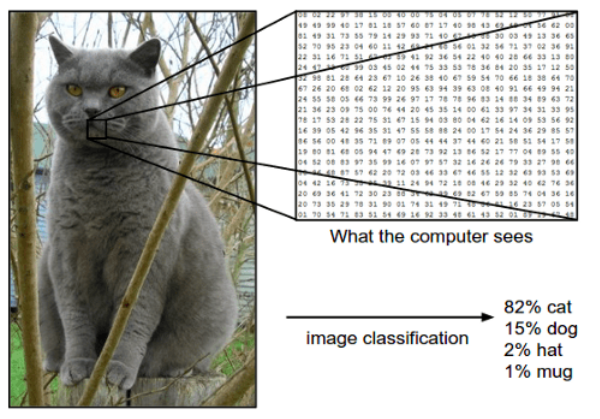
\includegraphics[width=1\linewidth]{images/how_computer_see_image}
	\caption[Cách máy tính "nhìn" một hình.]{Cách máy tính "nhìn" một hình ảnh.}
	%\label{fig:howcomputerseeimage}
\end{figure}

Convolutional Neural Networks (CNN) là một trong những mô hình deep learning phổ biến nhất và có ảnh hưởng nhiều nhất trong cộng đồng Computer Vision. CNN được dùng trong trong nhiều bài toán như nhân dạng ảnh, phân tích video, ảnh MRI, hoặc cho bài các bài của lĩnh vự xử lý ngôn ngữ tự nhiên, và hầu hết đều giải quyết tốt các bài toán này.

Mạng CNN lấy cảm hứng từ não người \cite{cnnhumanbrain}. Nghiên cứu trong những thập niên 1950 và 1960 của D.H Hubel và T.N Wiesel trên não của động vật đã đề xuất một mô hình mới cho việc cách mà động vật nhìn nhận thế giới. Trong báo cáo, hai ông đã diễn tả 2 loại tế bào neural trong não và cách hoạt động khác nhau: tế bào đơn giản (simple cell – S cell) và tế bào phức tạp (complex cell – C cell). 

Năm 1980, Fukushima đề xuất mô hình mạng neural có cấp bậc gọi là neocognitron. Mô hình này dựa trên khái niệm về S cell và C cell. Mạn neocognitron có thể nhận diện mẫu dựa trên việc học hình dáng của đối tượng. 

Sau đó vào năm 1998, mạng CNN được giới thiệu bởi Bengio, Le Cun, Bottou và Haffner. Mô hình đầu tiên của họ được gọi tên là LeNet-5. Mô hình này có thể nhận diện chữ số viết tay.

\subsection{Kiến trúc mạng CNN}
Mạng CNN gồm hai thành phần:

\indent\indent \textbf{Phần tầng ẩn hay phần rút trích đặc trưng:} trong phần này, mạng sẽ tiến hành tính toán hàng loạt phép tích chập và phép hợp nhất (pooling) để phát hiện các đặc trưng.

\indent\indent  \textbf{Phần phân lớp:} tại phần này, một lớp với các liên kết đầy đủ sẽ đóng vai trò như một bộ phân lớp các đặc trưng đã rút trích được trước đó. Tầng này sẽ đưa ra xác suất của một đối tượng trong hình \ref{fig:kientruccnn}.
\begin{figure}[H]
	\centering
	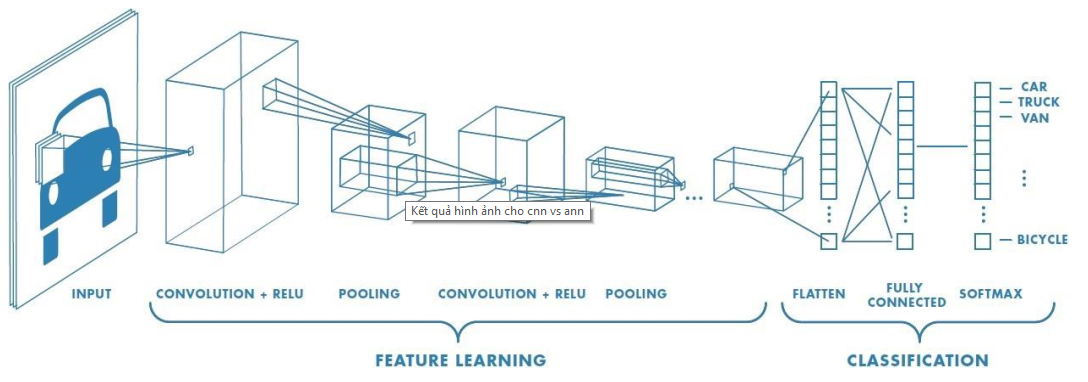
\includegraphics[width=1\linewidth]{images/kientruccnn}
	\caption{Kiến trúc mạng CNN.}
	\label{fig:kientruccnn}
\end{figure}

\subsubsection{Trích rút đặc trưng}
\paragraph{Lớp tích chập}
Tích chập là một khối quan trọng trong CNN. Thuật ngữ tích chập được dựa trên một phép hợp nhất toán học của hai hàm tạo thành hàm thứ ba. Phép toán này kết hợp hai tập thông tin khác nhau.

Trong trường hợp CNN, tích chập được thực hiện trên giá trị đầu vào của dữ liệu và kernel/filter (thuật ngữ này được sử dụng khác nhau tùy tình huống) để tạo ra một bản đồ đặc trưng (feature map). 

Ta thực hiện phép tích chập bằng cách trượt kernel/filter theo dữ liệu đầu vào. Tại mỗi vị trí, ta tiến hành phép nhân ma trận và tính tổng các giá trị để đưa vào bản đồ đặc trưng. Thao tác này đã được minh họa cụ thể trong hình \ref{fig:padding18}

\begin{figure}[H]
	\centering
	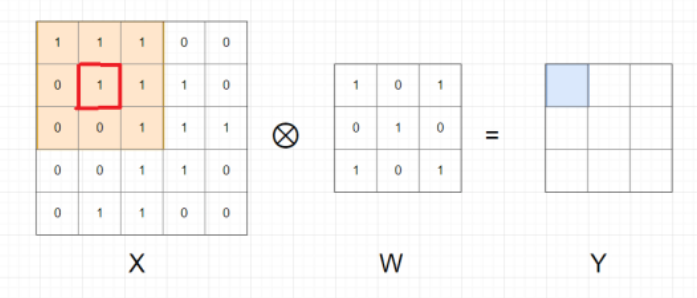
\includegraphics[width=1\linewidth]{images/padding18.png}
	\caption{Minh họa phép tích chập.}
	\label{fig:padding18}
\end{figure}

\paragraph{Lớp ReLU}

Tương tự như mạng neural thông thường, ta sử dụng một hàm kích hoạt (activate function) để có đầu ra dưới dạng phi tuyến. Trong trường hợp CNN, đầu ra của phép tích chập sẽ đi qua hàm kích hoạt nào đó ví dụ như hàm tinh chỉnh các đơn vị tuyến tính (Rectified linear units - ReLU). 

\paragraph{Lớp pooling}

Thông thường, sau mỗi tầng tích chập, ta sẽ cho kết quả đi qua một tầng hợp nhất (pooling layer). Mục đích của tầng này là để nhanh chóng giảm số chiều. Việc này giúp giảm thời gian học và hạn chế việc overfitting. 


Như vậy, khi thiết kế phần rút trích đặc trưng của mạng CNN, ta cần chú ý đến 4 siêu tham số quan trọng là: Kích thước kernel/filter, Số lượng kernel/filter, Kích thước bước nhảy (stride), Kích thước lề (padding).

\subsubsection{Phân lớp}
Tầng cuối cùng trong mạng CNN là một tầng liên kết đầy đủ, phần này hoạt động tương tự như mạng neural thông thường. Kết quả thu được cuối cùng cũng sẽ là một véc-tơ với các giá trị xác suất cho việc dự đoán như mạng neural thông thường.

\subsection{Ứng dụng CNN trong phân loại ảnh}
Các bước để thực hiện phân loại hình ảnh dựa trên mạng CNN được mô tả trong Hình \ref{fig:placnn}. Đầu tiên, kho dữ liệu ảnh đầu vào được nạp. Ảnh này được chia làm hai phần, một phần dành cho luyện mạng và một phần cho kiểm tra. Trước tiên, ta phải lựa chọn cấu trúc mạng CNN bao gồm số lượng lớp ẩn, các tham số trong mỗi lớp ẩn như kích thước trường tiếp nhận cục bộ, stride, padding.  Ảnh luyện mạng sau đó được đưa vào lớp chập 1 để thực hiện tích chập trên ảnh và thực hiện hàm ReLU. Sau đó, kết quả được đưa đến quá trình thực hiện pooling với tham số pooling size phù hợp để giảm kích cỡ ảnh. Ảnh sẽ tiếp tục được đưa thêm qua các lớp tích chập nữa cho đến khi đạt được kết quả mong muốn. Kết quả này được dàn phẳng và đưa vào lớp kết nối đầy đủ. Cuối cùng là quá trình thực hiện các activation function và phân loại ảnh. Quá trình luyện mạng sẽ kết thúc sau khi tổng sai số nhỏ hơn một ngưỡng cho phép hoặc sau một số thế hệ cho trước (điều kiện hội tụ). Kết thúc của quá trình luyện mạng là cấu trúc mạng CNN với các tham số phù hợp. Để kiểm tra, các mẫu ảnh kiểm tra được đưa qua mạng CNN rồi thực hiện đánh giá sai số.

\subsubsection{Trường tiếp nhận cục bộ (Local receptive fields)}
Là một cửa sổ nhỏ trên các điểm ảnh đầu vào. Mỗi kết nối sẽ học một trọng số và neural ẩn cũng sẽ học một độ lệch (overall bias). Ta có thể hiểu rằng, neural lớp ẩn cụ thể học để phân tích trường tiếp nhận cục bộ cụ thể của nó.

Có thể thấy rằng, trường tiếp nhận cục bộ thích hợp cho việc phân tách dữ liệu ảnh, giúp chọn ra những vùng ảnh có giá trị nhất cho việc đánh giá phân lớp.

\subsubsection{Trọng số chia sẻ và độ lệch (Shared weights and biases)}
Chúng ta gọi việc map từ input layer sang hidden layer là một feature map. Ta cần tìm ra mối quan hệ giữa số lượng Feature map với số lượng tham số.

Chúng ta thấy mỗi fearture map cần 25 = 5×5 shared weight và 1 shared bias. Như vậy mỗi feature map cần 5×5+1 = 26 tham số. Như vậy nếu có 10 feature map thì có 10×26 = 260 tham số. Chúng ta xét lại nếu layer đầu tiên có kết nối đầy đủ nghĩa là chúng ta có 28×28=784 neural đầu vào như vậy ta chỉ có 30 neural ẩn. Như vậy ta cần 28x28x30 shared weight và 30 shared bias. Mô hình có số lượng tham số ít hơn thì nó sẽ chạy nhanh hơn.

\subsubsection{Lớp chứa hay lớp tổng hợp (Pooling layer)}
Ngoài các lớp tích chập vừa mô tả, mạng neural tích chập cũng chứa các lớp pooling. Lớp pooling thường được sử dụng ngay sau lớp tích chập. Những gì các lớp pooling làm là đơn giản hóa các thông tin ở đầu ra từ các lớp tích chập. 

Chúng ta có thể hiểu max-pooling như là một cách cho mạng để hỏi xem một đặc trưng nhất được tìm thấy ở bất cứ đâu trong một khu vực của ảnh. Sau đó nó bỏ đi những thông tin định vị chính xác. Trực giác là một khi một đặc trưng đã được tìm thấy, vị trí chính xác của nó là không quan trọng như vị trí thô của nó so với các đặc trưng khác. Một lợi ích lớn là có rất nhiều tính năng gộp ít hơn (fewer pooled features), và vì vậy điều này sẽ giúp giảm số lượng các tham số cần thiết trong các lớp sau.

\subsubsection{Cách chọn tham số cho CNN}
Hiệu quả hoạt động của mạng CNN phụ thuộc rất nhiều vào việc lựa chọn các tham số sau:

\begin{itemize}
	\item Số các convolution layer: càng nhiều các convolution layer thì performance càng được cải thiện. Sau khoảng 3 hoặc 4 layer, các tác động được giảm một cách đáng kể.
	\item Filter size: thường filter theo size 5×5 hoặc 3×3
	\item Pooling size: thường là 2×2 hoặc 4×4 cho ảnh đầu vào lớn
\end{itemize}

Trong thực tế, tùy vào ứng dụng cụ thể mà ta chọn các tham số khác nhau. Thông thường ta sẽ thực hiện nhiều lần việc train test để chọn ra được param tốt nhất (Phương pháp thử sai).

\section{Bài toán chuẩn đoán bệnh lao}
\subsection{Các dữ liệu để chuẩn đoán bệnh lao}
Để chuẩn đoán được bệnh lao cần dựa vào rất nhiều dữ liệu \cite{bytchuandoanlao} như: 
\begin{itemize}
	\item {\bfseries Lâm sàng}
	\begin{itemize}
		\item {\bfseries Toàn thân:} Sốt nhẹ về chiều, ra mồ hôi đêm, chán ăn, mệt mỏi, gầy sút cân.
		\item {\bfseries Cơ năng:} Ho, khạc đờm, ho ra máu, đau ngực, khó thở.
		\item {\bfseries Thực thể:} Nghe phổi có thể có tiếng bệnh lý (ran ẩm, ran nổ,....).
	\end{itemize}
	\item {\bfseries Cận lâm sàng}
	\begin{itemize}
		\item Nhuộm soi đờm trực tiếp tìm AFB.
		\item Xét nghiệm Xpert MTB/RIF (nếu có thể).
		\item Nuôi cấy tìm vi khuẩn lao.
		\item X-Quang phổi thường quy.
	\end{itemize}
\end{itemize}

Tuy vậy, do mục tiêu, đối tượng nghiên cứu, phạm vi nghiên cứu, nên luận văn chỉ tập trung nghiên cứu hỗ trợ chuẩn đoán bệnh lao qua các hình ảnh x-quang phổi thường quy dựa vào học máy, học sâu.

\subsection{Mô tả bài toán}
Như đã đề cập ở trên, luận văn chỉ tập trung nghiên cứu hỗ trợ chuẩn đoán bệnh lao qua các hình ảnh x-quang phổi thường quy dựa vào học máy, học sâu nên bài toán này chính là bài toán phân loại ảnh trong Thị giác Máy - Computer Vision.

Bài toán phân loại hình ảnh của luận văn là một trong những nhiệm vụ phổ biến trong Computer Vision. Mục tiêu chính của bài toán này đó chính là phân loại một hình ảnh đầu vào (input) thành một nhãn (label) đầu ra (output).  

Sau đó, ta sẽ tiến hành huấn luyện các mô hình học sâu của luận văn. Sau khi hoàn thành quá trình huấn luyện, ta có thể để các mô hình đã được huấn luyện kể trên thực hiện nhiêm vụ phân loại, dự đoán về khả năng ảnh x-quang phổi được đưa vào là của người có lao hay không, đây là nhãn (label) đầu ra (output) mong muốn cho bài toán của luận văn, dựa vào nhãn đầu ra ta sẽ kết luận xem người có ảnh chụp x-quang đó có bị lao hay tổn thương phổi không. 
	\setcounter{chapter}{1}
\setcounter{section}{1}
\chapter{\tenchuongii}
%===================================================================
Từ mạng CNN cơ bản người ta có thể tạo ra rất nhiều mô hình khác nhau, từ những mạng neural cơ bản 1 đến 2 layer đến 100 layer. Khi thêm nhiều layer hơn thì theo lý thuyết độ chính xác phải cao hơn, nhưng thực tế lại không phải độ chính xác không tăng thậm chí là có lúc lại giảm. Về kernel ta có 3x3, 5x5 hay thậm chí 7x7, vậy thì dùng kernel nào tốt, càng nhỏ liệu có càng chính xác? Vì vậy, chương này ta sẽ tìm hiểu một số mô hình nổi tiếng của CNN, các cài đặt, cấu hình của chúng và hướng áp dụng vào bài toán chuẩn đoán bệnh lao của luận văn.

\section{Mô hình VGG-16}
\subsection{Mô hình VGG16 là gì}
VGG là viết tắt của Visual Geometry Group; nó là một kiến trúc CNN sâu tiêu chuẩn với nhiều lớp. Karen Simonyan và Andrew Zisserman \cite{vgg16} đã đề xuất ý tưởng về mạng VGG vào năm 2013 và gửi mô hình thực tế dựa trên ý tưởng này trong ImageNet Challenge 2014. Họ gọi nó là VGG theo tên bộ phận của Visual Geometry Group tại Đại học Oxford nơi họ làm việc.

\subsection{Cấu hình mô hình VGG16}
Trong tất cả các cấu hình, VGG16 được xác định là mô hình hoạt động tốt nhất trên tập dữ liệu ImageNet. Hãy xem lại kiến trúc thực tế của cấu hình này (Hình \ref{fig:vgg16_imagenet}).
Đầu vào cho bất kỳ cấu hình mạng nào được coi là hình ảnh có kích thước cố định 224 x 224 với ba kênh R, G và B. Quá trình xử lý trước duy nhất được thực hiện là chuẩn hóa các giá trị RGB cho mỗi pixel. Điều này đạt được bằng cách trừ đi giá trị trung bình cho mỗi pixel.

Hình ảnh được chuyển qua ngăn xếp đầu tiên gồm 2 lớp tích chập có kích thước tiếp nhận rất nhỏ là 3 x 3, tiếp theo là kích hoạt ReLU. Mỗi lớp trong số hai lớp này chứa 64 bộ lọc. Stride được cố định ở 1 pixel và padding là 1 pixel. Cấu hình này bảo toàn độ phân giải không gian và kích thước của bản đồ kích hoạt đầu ra giống với kích thước hình ảnh đầu vào. Các bản đồ kích hoạt sau đó được chuyển qua tổng hợp tối đa không gian trên cửa sổ 2 x 2 pixel, với stride là 2 pixel. Điều này làm giảm một nửa kích thước của các lần kích hoạt. Do đó, kích thước của các kích hoạt ở cuối ngăn xếp đầu tiên là 112 x 112 x 64.

Các kích hoạt sau đó chảy qua ngăn xếp thứ hai tương tự, nhưng với 128 bộ lọc so với 64 bộ lọc trong ngăn xếp thứ nhất. Do đó, kích thước sau ngăn xếp thứ hai trở thành 56 x 56 x 128. Tiếp theo là ngăn xếp thứ ba với ba lớp chập và một lớp tổng hợp tối đa. Số lượng bộ lọc được áp dụng ở đây là 256, làm cho kích thước đầu ra của ngăn xếp là 28 x 28 x 256. Tiếp theo là hai ngăn xếp gồm ba lớp chập, với mỗi ngăn chứa 512 bộ lọc. Đầu ra ở cuối cả hai ngăn xếp này sẽ là 7 x 7 x 512.

Các chồng lớp chập trùng được theo sau bởi ba lớp được kết nối hoàn chỉnh với một lớp làm phẳng ở giữa. Hai lớp đầu tiên có 4.096 tế bào thần kinh mỗi lớp và lớp được kết nối đầy đủ cuối cùng đóng vai trò là lớp đầu ra và có 1.000 tế bào thần kinh tương ứng với 1.000 lớp có thể có cho tập dữ liệu ImageNet. Tiếp theo là lớp đầu ra là lớp kích hoạt Softmax được sử dụng để phân loại (Hình \ref{fig:vgg16_imagenet_detail}).

\begin{figure}[H]
	\centering
	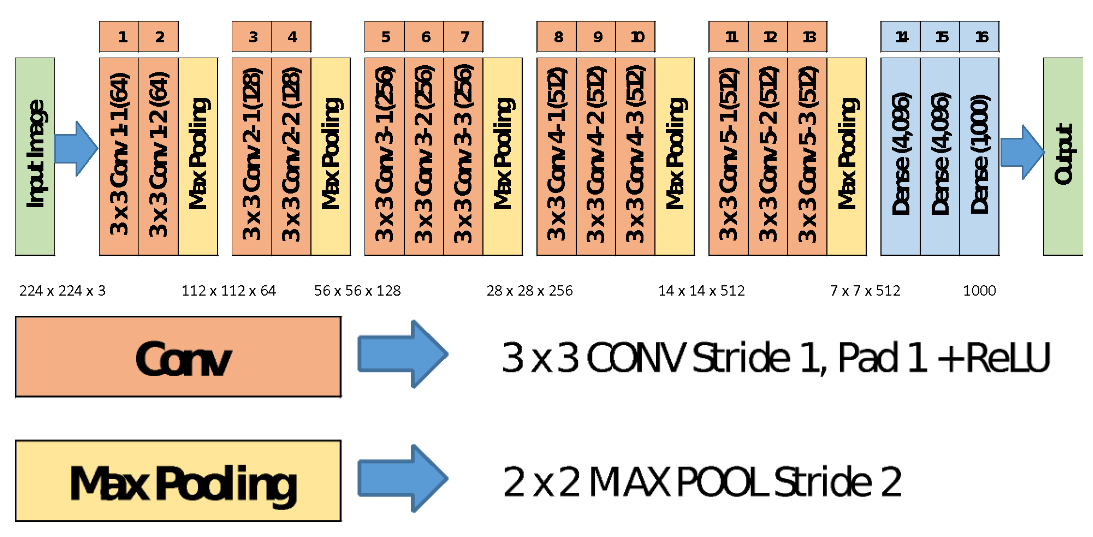
\includegraphics[width=1\linewidth]{images/vgg16_imagenet_detail}
	\caption{Chi tiết kiến trúc VGG16.}
	\label{fig:vgg16_imagenet_detail}
\end{figure}

\subsection{Ưu nhược điểm của mô hình VGG16}
\textbf{Ưu điểm:}
\begin{itemize}
	\item VGG đã mang đến một sự cải tiến lớn về độ chính xác và cải thiện cả về tốc độ. Điều này chủ yếu là do cải thiện độ sâu của mô hình.
	\item Sự gia tăng số lượng các lớp với các hạt nhân nhỏ hơn làm tăng tính phi tuyến tính, điều này luôn luôn là một điều tích cực trong học sâu.
	\item VGG mang theo nhiều kiến trúc khác nhau được xây dựng dựa trên khái niệm tương tự. Điều này cung cấp cho chúng ta nhiều lựa chọn hơn về kiến trúc nào có thể phù hợp nhất với ứng dụng của chúng ta.
\end{itemize}
\textbf{Nhược điểm:}
\begin{itemize}
	\item Một vấn đề của VGG liên quan đến giới hạn tính toán của máy tính cũng khiến cho việc huấn luyện không hiệu quả khi số lượng hidden layers lớn lên. Vấn đề này có tên là vanishing gradient.
	\item Số lượng bộ lọc mà chúng ta có thể sử dụng tăng gấp đôi trên mỗi bước hoặc qua mỗi ngăn xếp của lớp tích chập. Đây là một nguyên tắc chính được sử dụng để thiết kế kiến trúc của mạng VGG16. Một trong những nhược điểm quan trọng của mạng VGG16 là nó là một mạng khổng lồ, có nghĩa là cần nhiều thời gian hơn để đào tạo các tham số của nó.
\end{itemize}


\section{Mô hình ResNet}
\subsection{Mô hình Resnet là gì}
ResNet (Residual Network) được Kaiming He\cite{resnet} giới thiệu đến công chúng vào năm 2015, hiện tại thì có rất nhiều biến thể của kiến trúc ResNet với số lớp khác nhau như ResNet-18, ResNet-34, ResNet-50, ResNet-101, ResNet-152,... với tên là ResNet theo sau là một số chỉ kiến trúc ResNet với số lớp nhất định.

Các kiến trúc mạng trước khi Resnet ra đời như Alexnet, VGG được coi là các mạng nơ ron thuần (plain network). Đối với các mạng nơ ron thuần, Kaiming He\cite{resnet} đã thí nghiệm và đưa ra kết luận khi tăng số lượng layer của mạng từ 20 lên 56 thì lỗi trên tập huấn luyện và trên tập kiểm tra của mạng 56 layer đều cao hơn so với mạng 20 layer(hình \ref{fig:resnet_vanishing_gradient}). 
\begin{figure}[H]
	\centering
	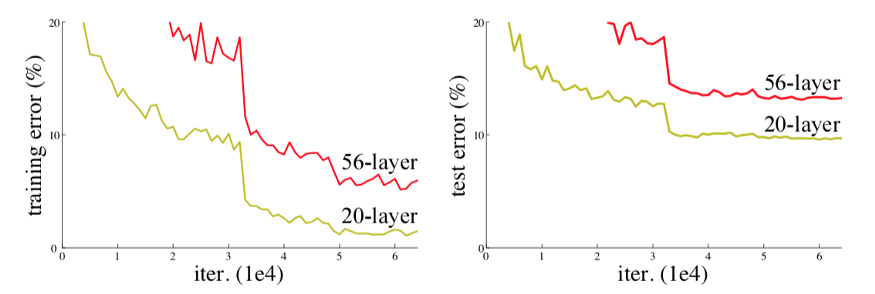
\includegraphics[width=1\linewidth]{images/resnet_vanishing_gradient}
	\caption{Lỗi huấn luyện và lỗi kiểm tra với mạng 20 layer và 56 layer.}
	\label{fig:resnet_vanishing_gradient}
\end{figure} 
ResNet đưa ra phương phán cho vấn đề trên là sử dụng kết nối "tắt" đồng nhất để xuyên qua một hay nhiều lớp. Một khối như vậy được gọi là một Residual Block(hình \ref{fig:resnet_residual_block}). Ý tưởng chính của phương pháp này thực ra rất đơn giản, Resnet thực hiện residual mapping để copy thông tin từ các layer nông shallow layer trước đó đến các layer sâu hơn. Chúng ta giả sử output của shallow layer là $x$. Trong quá trình forward của mạng nó được đưa qua một phép biến đổi tuyến tính $F(x)$. Chúng ta giả sử output của phép biến đổi tuyền tính này là $H(x)$. Một residual (phần dư) giữa deep layer và shallow layer là
$$\mathcal{F}(\mathbf{x}; W_i) := \mathcal{H}(\mathbf{x}) - \mathbf{x}$$
Trong đó, $W_i$ là các tham số của mô hình CNN với phép biến đổi $F$ và nó được tối ưu trong quá trình huấn luyện.
\begin{figure}[H]
	\centering
	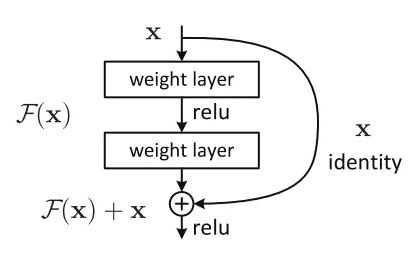
\includegraphics[width=0.5\linewidth]{images/resnet_residual_block}
	\caption{Residual block.}
	\label{fig:resnet_residual_block}
\end{figure}
Việc thêm vào các residual block vào trong kiến trúc mạng deep learning có hai cách tuỳ thuộc vào từng trường hợp cụ thể.
\begin{itemize}
	\item {\bf identity mapping} trong trường hợp này residual mapping đơn giản là việc cộng trực tiếp $x$ vào đầu ra của các stacked block $F(x)$. Đây là một cách sử dụng khá phổ biến trong thiết kế mạng ResNet nếu như input activation có cùng số chiều với output activation.
	\begin{figure}[H]
		\centering
		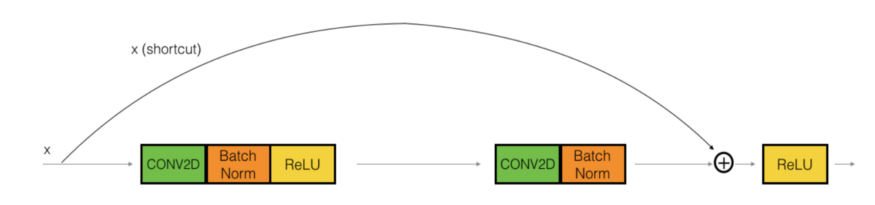
\includegraphics[width=1\linewidth]{images/resnet_identity_mapping}
		\caption{Identity mapping.}
		\label{fig:resnet_identity_mapping}
	\end{figure}
	\item {\bf Convolutional block} một trường hợp khác là thay vì cộng trực tiếp giá trị của input activation chúng ta sẽ đưa qua một convolution transformation. Trường hợp này có thể được thực hiện trong trường hợp input activation và output activation có số chiều khác nhau. Lúc này đầu ra được xác định như sau $y=F(x;Wi)+\text{Conv}(x)$.
	\begin{figure}[H]
		\centering
		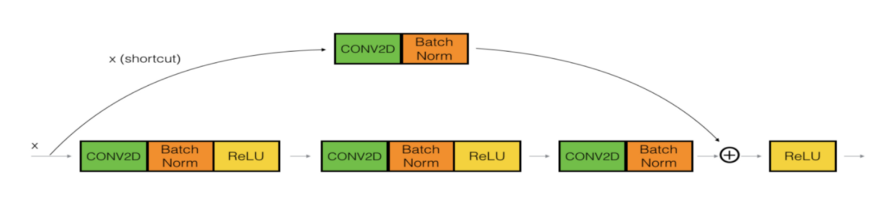
\includegraphics[width=1\linewidth]{images/resnet_conv_block}
		\caption{Convolutional block.}
		\label{fig:resnet_conv_block}
	\end{figure}
\end{itemize}
\subsection{Cấu hình của mô hình Resnet}
Hình \ref{fig:resnet_architecture} dưới đây mô tả chi tiết kiến trúc mạng nơ ron ResNet
\begin{figure}[H]
	\centering
	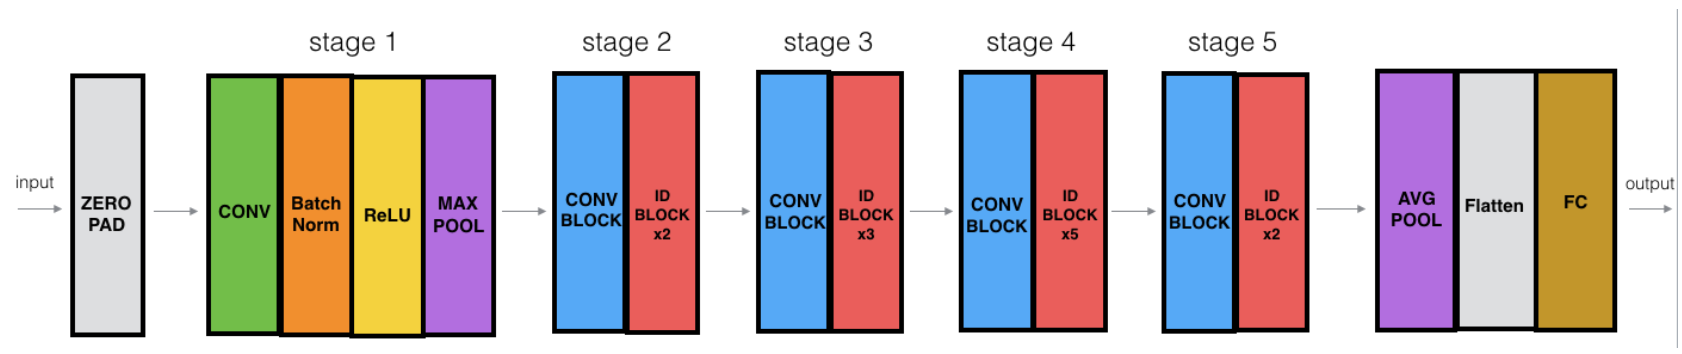
\includegraphics[width=1\linewidth]{images/resnet_architecture}
	\caption{Kiến trúc mạng ResNet.}
	\label{fig:resnet_architecture}
\end{figure}
"ID BLOCK" trong hình trên là viết tắt của từ Identity block và ID BLOCK x3 nghĩa là có 3 khối Identity block chồng lên nhau. Nội dung hình \ref{fig:resnet_architecture} như sau:
\begin{itemize}
	\item Zero-padding : Input với (3,3)
	\item Stage 1 : Tích chập (Conv1) với 64 filters với shape(7,7), sử dụng stride (2,2). BatchNorm, MaxPooling (3,3).
	\item Stage 2 : Convolutiontal block sử dụng 3 filter với size 64x64x256, f=3, s=1. Có 2 Identity blocks với filter size 64x64x256, f=3.
	\item Stage 3 : Convolutional sử dụng 3 filter size 128x128x512, f=3,s=2. Có 3 Identity blocks với filter size 128x128x512, f=3.
	\item Stage 4 : Convolutional sử dụng 3 filter size 256x256x1024, f=3,s=2. Có 5 Identity blocks với filter size 256x256x1024, f=3.
	\item Stage 5 :Convolutional sử dụng 3 filter size 512x512x2048, f=3,s=2. Có 2 Identity blocks với filter size 512x512x2048, f=3.
	\item The 2D Average Pooling : sử dụng với kích thước (2,2).
	\item The Flatten.
	\item Fully Connected (Dense) : sử dụng softmax activation.
\end{itemize}


\subsection{Ưu nhược điểm của mô hình ResNet}
\textbf{Ưu điểm:}
\begin{itemize}
	\item Kiến trúc ResNet không cần phải kích hoạt tất cả các nơ-ron trong mọi epoch (một epoch được tính là khi chúng ta đưa tất cả dữ liệu trong tập train vào mạng neural network 1 lần). Điều này làm giảm đáng kể thời gian đào tạo và cải thiện độ chính xác. Khi một đặc trưng đã được học, nó sẽ không cố gắng học lại mà tập trung vào việc học các đặc trưng mới hơn. Một cách tiếp cận rất thông minh đã cải thiện đáng kể hiệu suất đào tạo mô hình.
	\item ResNets giải quyết được khá tốt vấn đề Vanishing Gradient của các mạng CNN thuần.
	\item Có thể đào tạo dễ dàng các mạng với số lớp rất lớn mà không làm tăng tỷ lệ đào tạo lỗi.
\end{itemize}
\textbf{Nhược điểm: \cite{resnet_disadvantage}}
\begin{itemize}
	\item Đối với mạng sâu hơn, việc phát hiện lỗi trở nên khó khăn.
	\item Nếu mạng quá nông, việc đào tạo có thể rất kém hiệu quả.
\end{itemize}

\section{Mô hình DenseNet}
\subsection{Mô hình DenseNet là gì}
DenseNet - Dense Convolutional Network (Mạng Tích chập Kết nối Dày đặc) - là một trong những biến thể mở rộng của Resnet và là một kiến trúc mạng,trong đó mỗi lớp được kết nối trực tiếp với mỗi lớp khác nhau theo kiểu chuyển tiếp (trong mỗi khối dense block). Đối với mỗi lớp, các bản đồ đặc trưng (feature map) của tất cả các lớp ở phần trước được coi là các đầu vào riêng biệt và ở đó các bản đồ tính năng lại tiếp tục làm đầu vào cho tất cả các lớp tiếp theo. 

\begin{figure}[H]
	\centering
	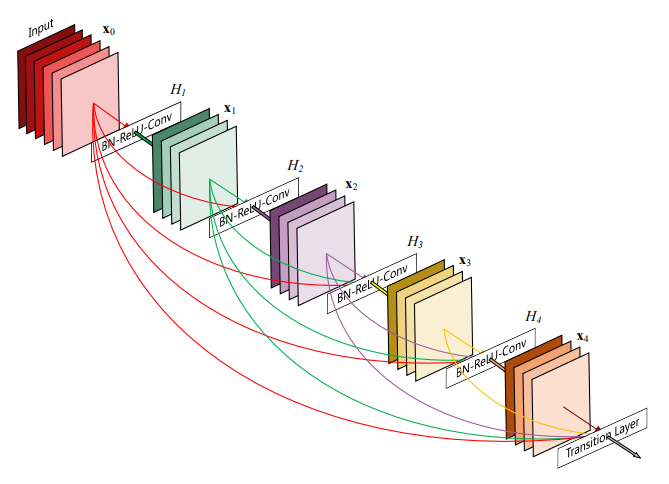
\includegraphics[width=0.8\linewidth]{images/densenet_hl}
	\caption{Kiến trúc DenseNet.}
	\label{fig:kien_truc_densenet}
\end{figure} 

Để cải thiện hơn nữa luồng thông tin giữa các lớp, DenseNet đề xuất một mô hình kết nối mà từ bất kỳ lớp nào cũng có thể kết nối đến tất cả các lớp tiếp theo. Hình \ref{fig:kien_truc_densenet} minh họa bố trí kiến trúc của DenseNet. Dễ dàng nhìn thấy, lớp thứ $l$ nhận được các bản đồ đặc trưng của tất cả các lớp trước đó, $x_0, x_1, x_2, . . . , x_{l-1}),$ làm đầu vào:
\begin{equation}\label{eq:denseconnectivity}
	x_l = H_l([x_0, x_1, . . . , x_{l-1}])
\end{equation}
với $[x_0, x_1, . . . , x{l-1}]$ đề cập đến việc nối các trích chọn đặc trưng được tạo thành trong các lớp $0, 1, ..., {l-1}$. Do khả năng kết nối dày đặc của nó, Gao Huang\cite{densenet} gọi kiến trúc mạng này là Mạng kết nối dày đặc (DenseNet). Để dễ thực hiện, DenseNet nối nhiều đầu vào của $H_l$(·) trong phương trình \ref{eq:denseconnectivity} thành một tensor duy nhất.\\
{\bf Hàm tổng hợp - Composite function}
Ta định nghĩa $H_l$(·) là một hàm tổng hợp của ba hoạt động liên tiếp: Batch Normalization (BN), tiếp theo là một hàm tinh chỉnh các đơn vị tuyến tính (ReLU) và một tích chập 3 × 3 (Conv).\\
{\bf Tầng hợp nhất - Pooling layers}
Thao tác nối được sử dụng trong Phương trình \ref{eq:denseconnectivity} không khả thi khi kích thước của bản đồ đối tượng thay đổi. Tuy nhiên, một phần thiết yếu của mạng tích chập là các lớp lấy mẫu xuống làm thay đổi kích thước của bản đồ đối tượng. Để tạo điều kiện thuận lợi cho việc giảm tần số lấy mẫu trong kiến trúc, DenseNet chia mạng thành nhiều khối dày đặc được kết nối với nhau(hình \ref{fig:densenet_3blk}). DensetNet đề cập đến các lớp giữa các khối là các lớp chuyển tiếp, các lớp này thực hiện tích chập và tổng hợp. Các lớp chuyển tiếp được sử dụng trong các cấu trúc DenseNet bao gồm lớp chuẩn hóa hàng loạt và lớp tích chập 1 × 1, tiếp theo là lớp gộp trung bình 2 × 2.
\begin{figure}[H]
	\centering
	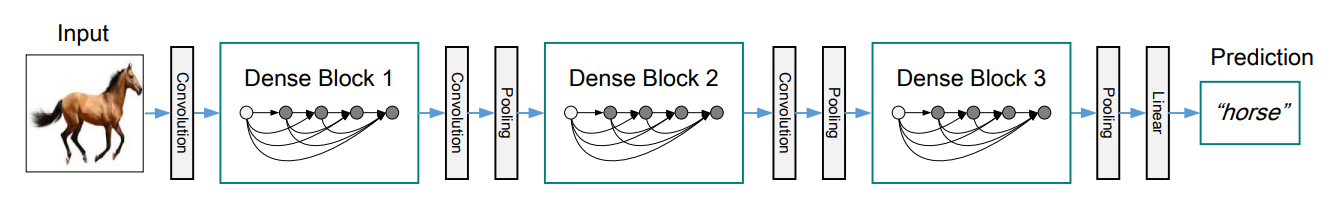
\includegraphics[width=1\linewidth]{images/densenet_3blk}
	\caption{Một DenseNet sâu với ba khối dày đặc.}
	\label{fig:densenet_3blk}
\end{figure}
{\bf Tỉ lệ phát triển - Growth rate}
Nếu mỗi hàm $H_l$ tạo ra $k$ bản đồ đặc trưng, thì lớp thứ $l$ có $k_0 + k{l-1}$ bản đồ đặc trưng đầu vào, trong đó $k_0$ là số kênh trong lớp đầu vào. Một điểm khác biệt quan trọng giữa DenseNet và các kiến trúc mạng trước đó là DenseNet có thể có các lớp rất hẹp, ví dụ: $k = 12$. Ta gọi siêu tham số $k$ là tỉ lệ phát triển của mạng. Tỉ lệ phát triển quy định lượng thông tin mới mà mỗi lớp đóng góp vào trạng thái toàn cục. Trạng thái toàn cục, sau khi được lưu trữ, có thể được truy cập từ mọi nơi trong mạng mà không cần phải sao chép nó từ lớp này sang lớp khác - không giống như trong các kiến trúc mạng truyền thống.\\
{\bf Các lớp nút cổ chai - Bottleneck layers}
Mặc dù mỗi lớp chỉ tạo ra $k$ bản đồ đặc trưng đầu ra, nhưng nó thường có nhiều đầu vào hơn. Người ta lưu ý rằng tích chập 1 × 1 có thể được đưa vào làm lớp nút cổ chai trước mỗi tích chập 3 × 3 để giảm số lượng bản đồ đặc trưng đầu vào và từ đó để cải thiện hiệu quả tính toán. Thiết kế này đặc biệt hiệu quả đối với DenseNet.\\
{\bf Độ nén - Compression}
Để cải thiện hơn nữa độ nhỏ gọn của mô hình, chúng ta có thể giảm số lượng bản đồ đặc trưng ở các lớp chuyển tiếp. Nếu một khối dày đặc chứa $m$ bản đồ đặc trưng, để lớp chuyển tiếp sau tạo ra $\theta m$ bản đồ đặc trưng đầu ra, trong đó $0 < \theta \leq 1$ được gọi là hệ số nén. Khi $\theta = 1$, số lượng bản đồ đối tượng trên các lớp chuyển tiếp không thay đổi.

\subsection{Cấu hình của mô hình DenseNet}
Từ hình \ref{fig:densenet_3blk}, có thể nhận thấy rằng DenseNets được chia thành nhiều khối dày đặc DenseBlock. Các kiến trúc khác nhau của DenseNets đã được tóm tắt trong bài báo "Densely Connected Convolutional Networks"\cite{densenet}. 

Mỗi kiến trúc bao gồm bốn DenseBlock với số lượng lớp khác nhau. Ví dụ, DenseNet-121 có [6,12,24,16] lớp trong bốn khối dày đặc trong khi DenseNet-169 có [6, 12, 32, 32] lớp. Chúng ta có thể thấy rằng phần đầu tiên của kiến trúc DenseNet bao gồm Lớp chuyển đổi 2 bước 7x7, tiếp theo là lớp MaxPooling 3x3 bước-2. Và khối dày đặc thứ tư được theo sau bởi một Lớp phân loại chấp nhận các bản đồ đặc trưng của tất cả các lớp của mạng để thực hiện phân loại. 

Ngoài ra, các phép toán tích chập bên trong mỗi kiến trúc là các lớp Cổ chai. Điều này có nghĩa là Conv 1x1 làm giảm số lượng kênh trong đầu vào và Conv 3x3 thực hiện hoạt động tích chập trên phiên bản đã biến đổi của đầu vào với số lượng kênh giảm hơn so với đầu vào.
\begin{figure}[H]
	\centering
	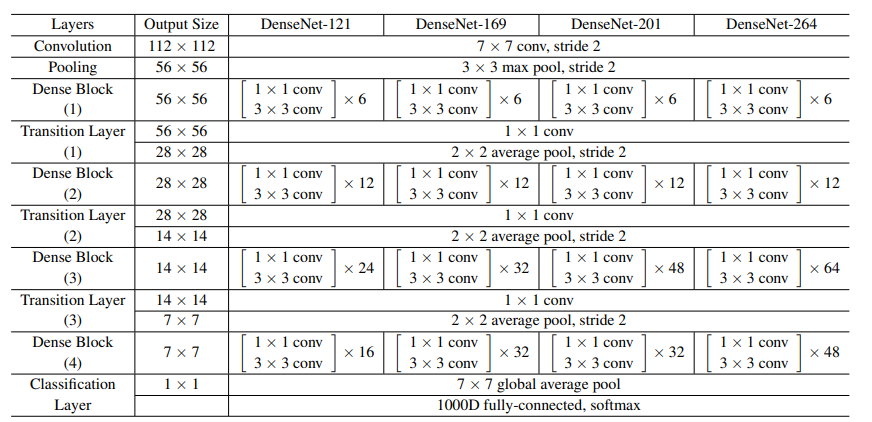
\includegraphics[width=1\linewidth]{images/densenet_archtectures_for_imagenet}
	\caption{Các kiến trúc DenseNet.}
	\label{fig:densenet_archtectures_for_imagenet}
\end{figure}

\subsection{Cài đặt mô hình DenseNet}
\begin{lstlisting}[language=Python]
def DenseNet(input_shape=(512, 512, 1),nb_dense_block=4, growth_rate=32, nb_filter=64, reduction=0.0, dropout_rate=0.0, weight_decay=1e-4, classes=1000, weights_path=None):

	eps = 1.1e-5
	
	compression = 1.0 - reduction
	
	global concat_axis
	concat_axis = 3
	img_input = Input(shape=input_shape, name='data')
	
	# From architecture for ImageNet (Table 1 in the paper)
	nb_filter = 64
	nb_layers = [6,12,24,16] # For DenseNet-121
	
	# Initial convolution
	x = ZeroPadding2D((3, 3), name='conv1_zeropadding')(img_input)
	x = Convolution2D(nb_filter, 7, 7, subsample=(2, 2), name='conv1', bias=False)(x)
	x = batch_normalization(epsilon=eps, axis=concat_axis, name='conv1_bn')(x)
	x = Activation('relu', name='relu1')(x)
	x = ZeroPadding2D((1, 1), name='pool1_zeropadding')(x)
	x = MaxPooling2D((3, 3), strides=(2, 2), name='pool1')(x)
	
	# Add dense blocks
	for block_idx in range(nb_dense_block - 1):
	stage = block_idx+2
	x, nb_filter = dense_block(x, stage, nb_layers[block_idx], nb_filter, growth_rate, dropout_rate=dropout_rate, weight_decay=weight_decay)
	
	# Add transition_block
	x = transition_block(x, stage, nb_filter, compression=compression, dropout_rate=dropout_rate, weight_decay=weight_decay)
	nb_filter = int(nb_filter * compression)
	
	final_stage = stage + 1
	x, nb_filter = dense_block(x, final_stage, nb_layers[-1], nb_filter, growth_rate, dropout_rate=dropout_rate, weight_decay=weight_decay)
	
	x = batch_normalization(epsilon=eps, axis=concat_axis, name='conv'+str(final_stage)+'_blk_bn')(x)
	x = Activation('relu', name='relu'+str(final_stage)+'_blk')(x)
	x = GlobalAveragePooling2D(name='pool'+str(final_stage))(x)
	
	x = Dense(classes, name='fc6')(x)
	x = Activation('softmax', name='prob')(x)
	
	model = Model(img_input, x, name='densenet')
	
	if weights_path is not None:
	model.load_weights(weights_path)
	
	return model
	
	
def conv_block(x, stage, branch, nb_filter, dropout_rate=None, weight_decay=1e-4):
	eps = 1.1e-5
	conv_name_base = 'conv' + str(stage) + '_' + str(branch)
	relu_name_base = 'relu' + str(stage) + '_' + str(branch)
	
	# 1x1 Convolution (Bottleneck layer)
	inter_channel = nb_filter * 4  
	x = batch_normalization(epsilon=eps, axis=concat_axis, name=conv_name_base+'_x1_bn')(x)
	x = Activation('relu', name=relu_name_base+'_x1')(x)
	x = Convolution2D(inter_channel, 1, 1, name=conv_name_base+'_x1', bias=False)(x)
	
	if dropout_rate:
	x = Dropout(dropout_rate)(x)
	
	# 3x3 Convolution
	x = batch_normalization(epsilon=eps, axis=concat_axis, name=conv_name_base+'_x2_bn')(x)
	x = Activation('relu', name=relu_name_base+'_x2')(x)
	x = ZeroPadding2D((1, 1), name=conv_name_base+'_x2_zeropadding')(x)
	x = Convolution2D(nb_filter, 3, 3, name=conv_name_base+'_x2', bias=False)(x)
	
	if dropout_rate:
	x = Dropout(dropout_rate)(x)
	
	return x
	
	
def transition_block(x, stage, nb_filter, compression=1.0, dropout_rate=None, weight_decay=1E-4):
	eps = 1.1e-5
	conv_name_base = 'conv' + str(stage) + '_blk'
	relu_name_base = 'relu' + str(stage) + '_blk'
	pool_name_base = 'pool' + str(stage) 
	
	x = batch_normalization(epsilon=eps, axis=concat_axis, name=conv_name_base+'_bn')(x)
	x = Activation('relu', name=relu_name_base)(x)
	x = Convolution2D(int(nb_filter * compression), 1, 1, name=conv_name_base, bias=False)(x)
	
	if dropout_rate:
	x = Dropout(dropout_rate)(x)
	
	x = AveragePooling2D((2, 2), strides=(2, 2), name=pool_name_base)(x)
	
	return x
	
	
def dense_block(x, stage, nb_layers, nb_filter, growth_rate, dropout_rate=None, weight_decay=1e-4, grow_nb_filters=True):
	concat_feat = x
	
	for i in range(nb_layers):
	branch = i+1
	x = conv_block(concat_feat, stage, branch, growth_rate, dropout_rate, weight_decay)
	concat_feat = merging([concat_feat, x], mode='concat', concat_axis=concat_axis, name='concat_'+str(stage)+'_'+str(branch))
	
	if grow_nb_filters:
	nb_filter += growth_rate
	
	return concat_feat, nb_filter
\end{lstlisting}

\subsection{Ưu nhược điểm của mô hình DenseNet}
\textbf{Ưu điểm:}
\begin{itemize}
	\item Giải quyết khá tốt vấn đề vanishing-gradient của các mạng CNN thuần.
	\item Cải thiện sự truyền tải đặc trưng giữa các lớp cả về phía trước cũng như phía sau.
	\item Giảm đáng kể số lượng tham số.
	\item Khuyến khích sử dụng lại các đặc trưng.
\end{itemize}
\textbf{Nhược điểm:}
\begin{itemize}
	\item Kết nối quá mức không chỉ làm giảm hiệu suất tính toán và hiệu quả tham số của mạng mà còn làm cho các mạng dễ bị overfitting. \cite{densenet_disadvantage}
\end{itemize}
	 
	 

	\setcounter{chapter}{2}
\setcounter{section}{1}
\chapter{\tenchuongiii}
\section{Phân tích yêu cầu bài toán}
Với bài toán phân loại ảnh của luận văn, ta có tập dữ liệu ảnh chụp x-quang phổi đã được gán nhãn làm hình ảnh đầu vào (input). Hình ảnh có định dạng PNG như hình \ref{fig:normalimg}.

Tập dữ liệu trên được một nhóm các nhà nghiên cứu từ Đại học Qatar, Doha, và Đại học Dhaka, Bangladesh cùng với các cộng tác viên của họ từ Malaysia phối hợp với các bác sĩ từ Hamad Medical Corporation và Bangladesh đã tạo ra một cơ sở dữ liệu về hình ảnh X-quang phổi cho người có lao cùng với hình ảnh người không có lao \cite{dataset}. Dữ liệu trên được cung cấp miễn phí tại \href{https://www.kaggle.com/datasets/tawsifurrahman/tuberculosis-tb-chest-xray-dataset}{https://www.kaggle.com/datasets/tawsifurrahman/tuberculosis-tb-chest-xray-dataset}. Thông tin cụ thể về tập dữ liệu như sau:
\begin{itemize}
	\item Tổng số 4200 ảnh đã được phân loại thành hai thư mục Normal (bình thường) và Tuberculosis (có lao).
	\item Số ảnh người mắc lao: 700 ảnh.
	\item Số ảnh người không mắc lao: 3500 ảnh.
	\item Kích thước ảnh: 512 x 512 (pixel)
	\item Định dạng ảnh: PNG.
	\item Tập tin Normal.metadata.xlsx tổng hợp thông tin về các file ảnh của người không mắc lao.
	\item Tập tin Tuberculosis.metadata.xlsx tổng hợp thông tin về các file ảnh của người mắc lao.
\end{itemize}

Mục tiêu mong muốn của bài toán là việc có thể dự đoán về khả năng ảnh x-quang phổi được đưa vào là của người có lao hay không, đây là nhãn (label) đầu ra (output) mong muốn, dựa vào nhãn đầu ra này ta sẽ kết luận xem người có ảnh chụp x-quang đó có bị lao hay tổn thương phổi không. Để thực hiện được mục tiêu trên, ta cần thực hiện hai pha:
\begin{itemize}
	\item \textbf{Học:} Lặp lại nhiều lần việc lần lượt đưa tất cả ảnh đầu vào để huấn luyện mô hình, trích chọn ra các đặc trưng của ảnh rồi lưu lại. Quá trình này nên dừng lại khi độ chính xác đạt mức tối thiểu mà ta đặt ra hoặc độ chính xác tăng lên không đáng kể sau một số lượt huấn luyện nhất định. 
	\item \textbf{Phân loại:} Dùng các đặc trưng mà mô hình thu được tại pha Học, đưa ảnh chụp x-quang đầu vào để tiến hành so sánh với các đặc trưng đó, kết thúc quá trình bằng một giá trị dự đoán khả năng mắc lao của người có ảnh x-quang được đưa vào.
\end{itemize}

\section{Phân tích lựa chọn công cụ}
\subsection{Lựa chọn mô hình đã hệ thống hóa}
Tại công bố của Karen Simonyan và Andrew Zisserman \cite{vgg16}, các tác giả có thông tin mạng VGG có số lượng tham số khổng lồ từ 133 - 144 triệu. Với hệ thống được hỗ trợ là bốn NVIDIA Titan Black GPUs, việc đào tạo một mô hình đơn chiếm tới 2-3 tuần tùy thuộc vào cấu trúc. Chính vì vấn đề thời gian và nguồn tài nguyên nghiên cứu không thể đáp ứng nên chương trình thử nghiệm sẽ không áp dụng mô hình VGG.
 
Tham khảo kết quả nghiên cứu được công bố của Gao Huang \cite{densenet}, tác giả so sánh tỷ lệ lỗi trên tập dữ liệu CIFAR và SVHN của các mô hình CNN, đặc biệt là mô hình ResNet và các biến thể của nó, ta dễ dàng nhận ra DenseNet có tỉ lể lỗi thấp hơn so với các mô hình ResNet, số lượng tham số cũng có ít hơn ResNet. Từ đây có thể nhận thấy rõ nên áp dụng mô hình DenseNet.

Chính vì những cơ sở trên, học viên quyết định sử dụng mô hình DenseNet cho phần mềm thử nghiệm của luận văn.

\subsection{Phân tích mô hình hệ thống}
Hệ thống chương trình thử nghiệm Phần mềm chuẩn đoán bệnh lao được thiết kế theo kiến trúc Client/Server năm tầng, trong đó:
\begin{itemize}
	\item {\bf Tầng thứ nhất} là tầng giao diện người phân loại, cụ thể là ứng dụng client trên trình duyệt, quản lý tương tác người phân loại với ứng dụng như chọn ảnh gửi lên server… và hiển thị kết quả phân loại do server gửi về.
	\item {\bf Tầng thứ hai} là tầng server quản lý cấu hình hệ thống, ví dụ cấu hình giao thức gửi/nhận dữ liệu với client, cụ thể giao thức được sử dụng trong hệ thống là giao thức HTTP.
	\item {\bf Tầng thứ ba} là tầng server thực hiện logic xử lý các yêu cầu từ client, như	quản lý và phân phối các luồng xử lý độc lập, đảm bảo hiệu năng và chất lượng tính toán phân loại cho nhiều client trong cùng một thời điểm.
	\item {\bf Tầng thứ tư} là tầng đảm nhiệm xây dựng, tinh chỉnh và quản lý các phiên	bản mô hình phân loại cho hệ thống, với bộ ảnh huấn luyện được lấy từ tầng quản lý dữ liệu bên dưới.
	\item {\bf Tầng cuối cùng} là tầng quản lý dữ liệu, bao gồm CSDL ảnh phục vụ cho việc huấn luyện mô hình, CSDL ảnh đã xử lý từ các client nhằm mục đích bổ sung sự	đa dạng của CSDL ảnh và cải thiện độ chính xác của mô hình phân loại. Các bộ ảnh trên được lưu tách biệt để thuận tiện cho việc quản lý và đánh giá độ chính xác của các
	phiên bản mô hình huấn luyện cũng như mức độ ảnh hưởng của bộ ảnh huấn luyện lên chất lượng mô hình.
\end{itemize}


\section{Một số kết quả chương trình}
\subsection{Một số giao diện và chức năng chính chính của chương trình}
\subsection{Giao diện đăng nhập hệ thống}
Giao diện đăng nhập hệ thống cung cấp lớp bảo vệ cơ bản cùng khả năng định danh người dùng, từ đó đưa ra nhưng ngữ cảnh thực đơn phù hợp.
\begin{figure}[H]
	\centering
	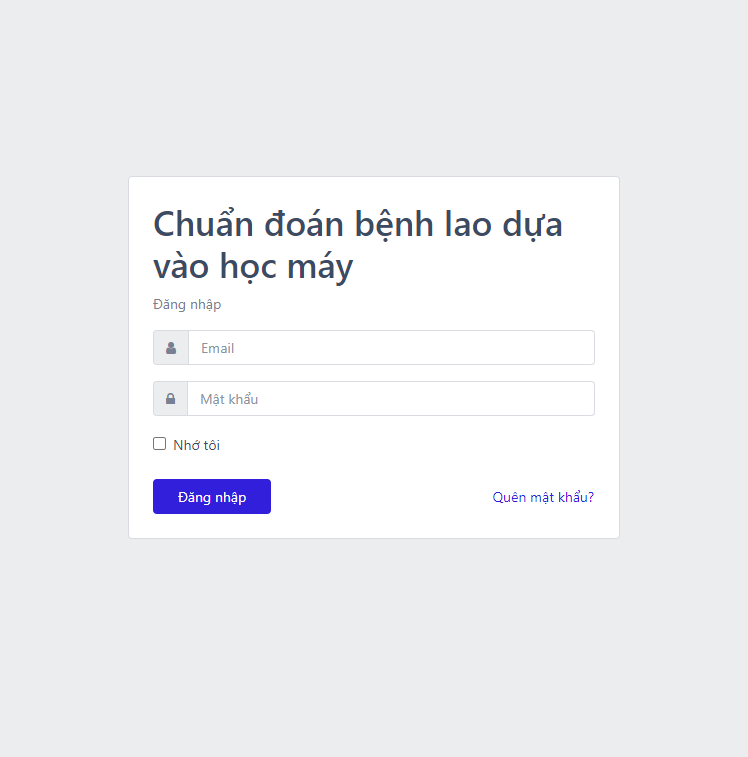
\includegraphics[width=1\linewidth]{images/giaodien_dangnhap}
	\caption{Giao diện đăng nhập hệ thống.}
	\label{fig:giaodien_dangnhap}
\end{figure}

\subsubsection{Giao diện cập nhật mô hình}
Tại đây, quản trị viên có thể thay đổi mô hình được sử dụng trong hệ thống. Mô hình này là được tạo ra ở pha Học. Mô hình mới được tải lên server, lưu trữ lại và ghi lại thông tin về đường dẫn để hệ thống có thể gọi được khi cần thiết.
\begin{figure}[H]
	\centering
	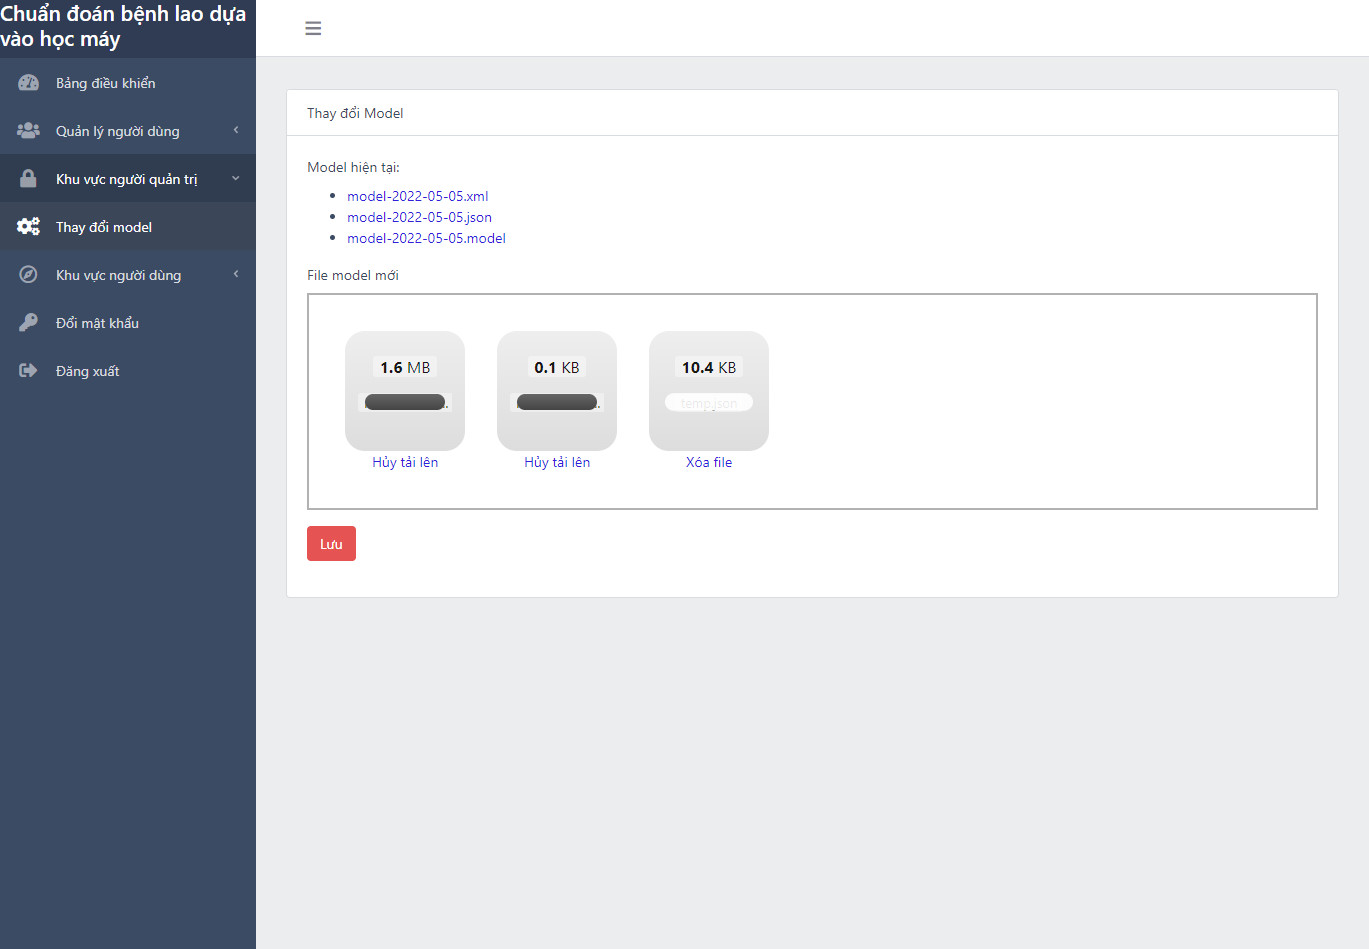
\includegraphics[width=1\linewidth]{images/quantri_doi_model}
	\caption{Giao diện cập nhật mô hình được sử dụng của hệ thống.}
	\label{fig:quantri_doi_model}
\end{figure}

\subsubsection{Giao diện danh sách các dự đoán}
Giao diện này tập trung thông tin của tất cả các dự đoán đã được thực hiện và lưu lại của hệ thống. Hệ thống sẽ hiện thị tất cả các dự đoán đối với người quản trị, và với tài khoản người dùng, hệ thống chỉ hiển thị những dự đoán thuộc về người dùng.
\begin{figure}[H]
	\centering
	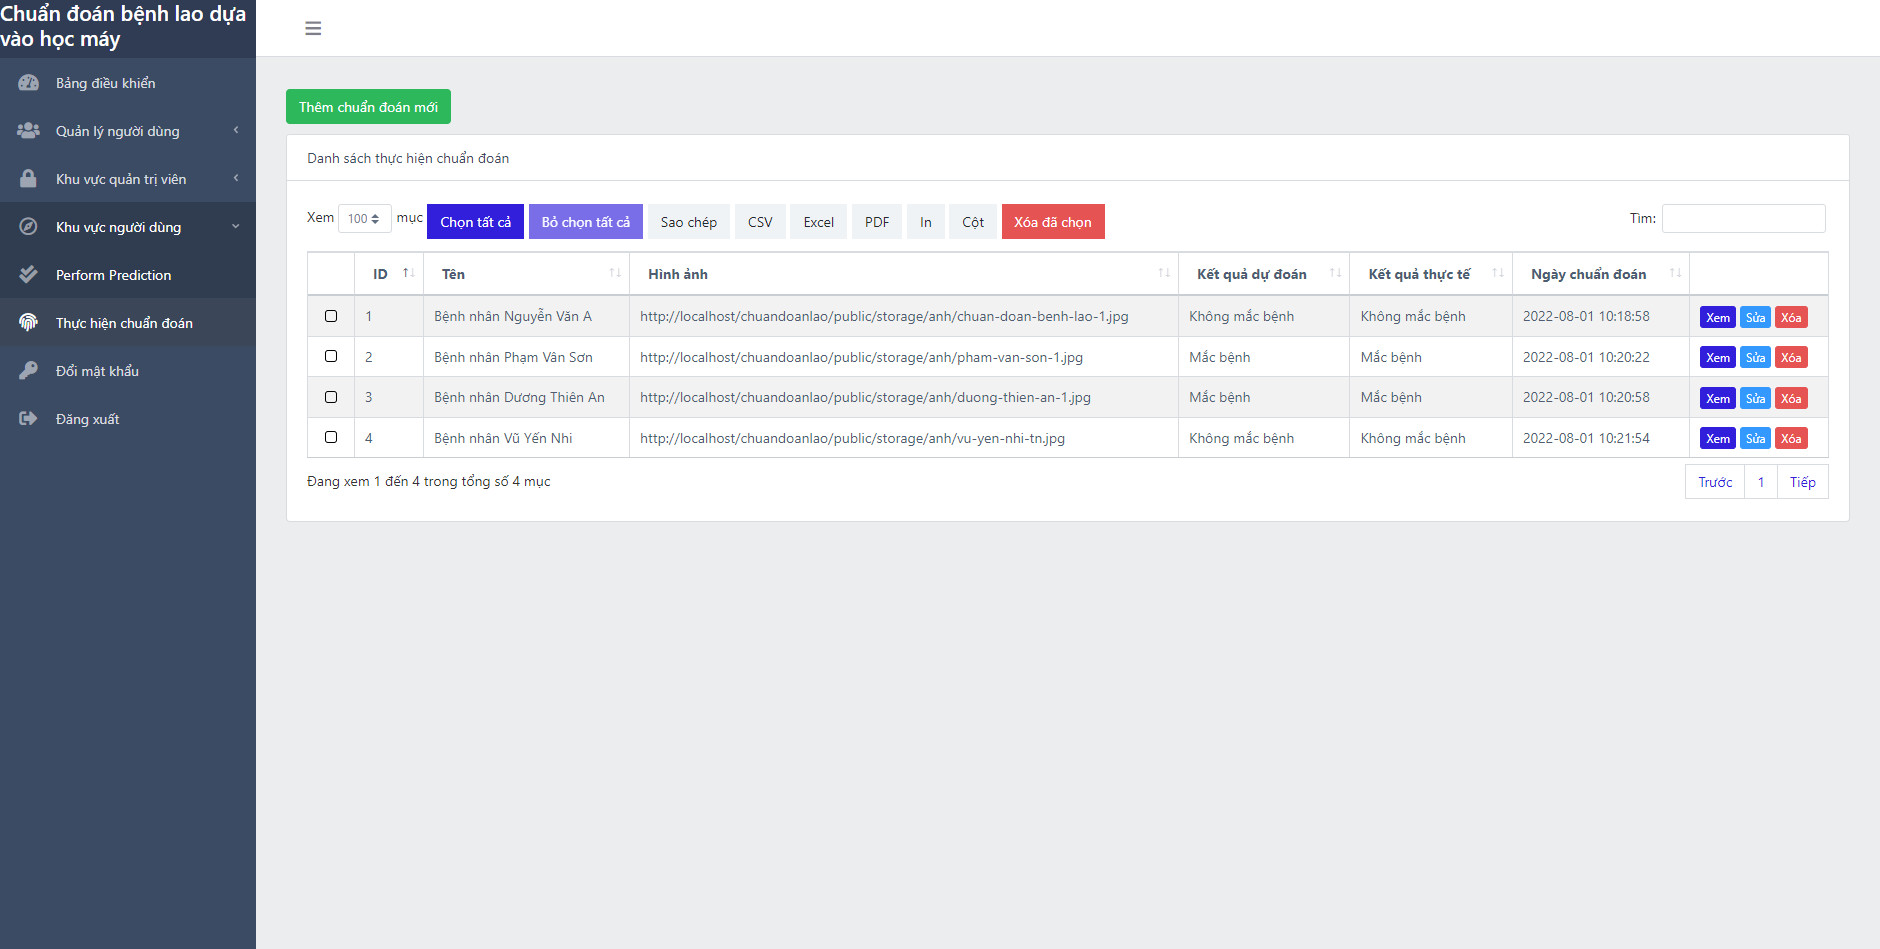
\includegraphics[width=0.95\linewidth]{images/user_danh_sach}
	\caption{Giao diện danh sách các dự đoán của hệ thống.}
	\label{fig:user_danh_sach}
\end{figure}

\subsection{Giao diện thực hiện dự đoán}
Người dùng upload ảnh chụp x-quang đã chuyển đổi định dạng PNG với kích thước 512x512 tại đây và nhận về kết quả dự đoán.
\begin{figure}[H]
	\centering
	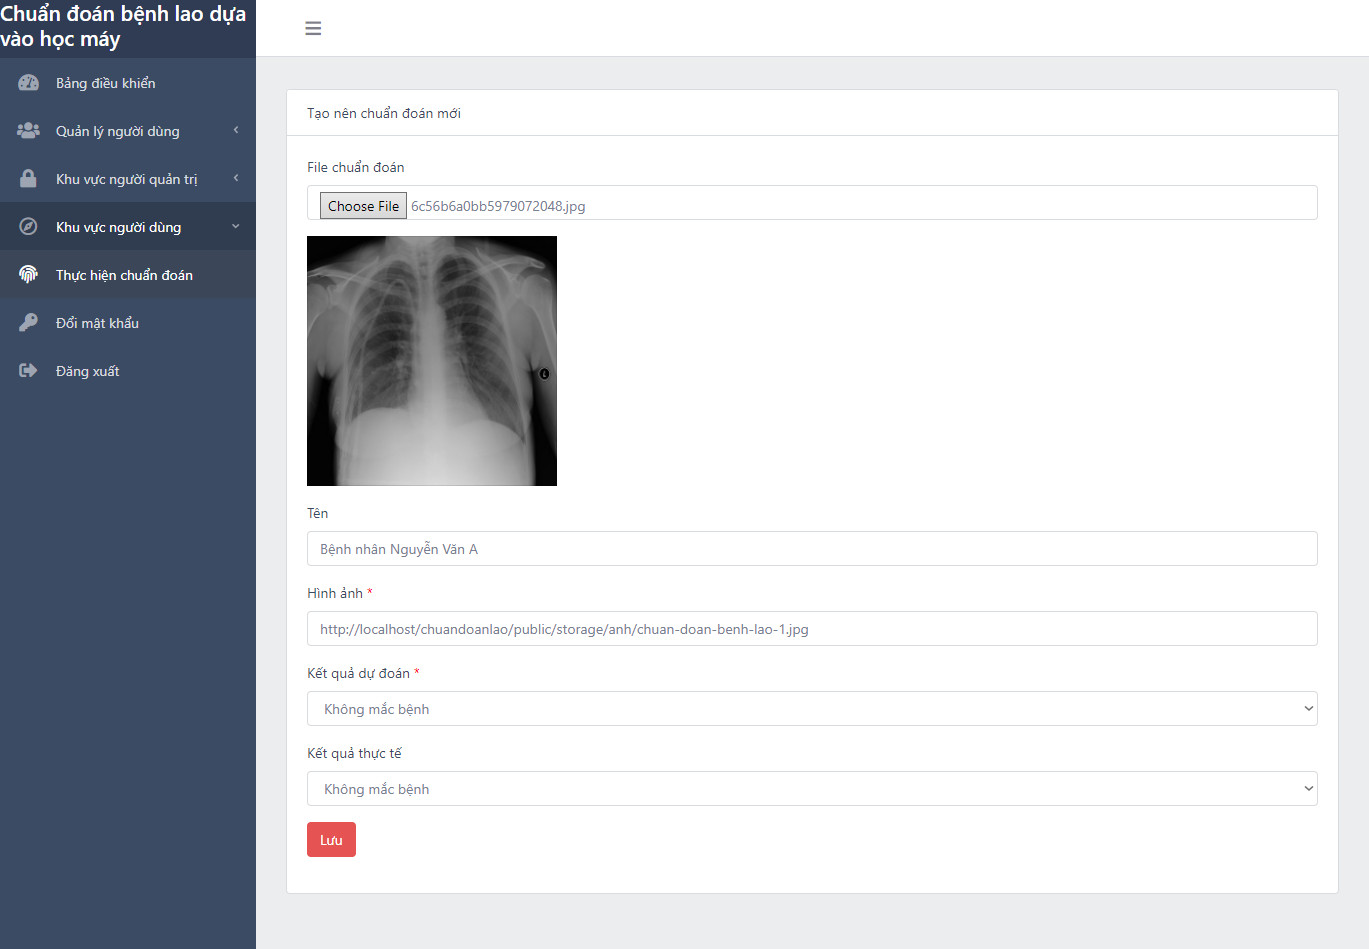
\includegraphics[width=0.95\linewidth]{images/user_du_doan_chi_tiet}
	\caption{Giao diện thực hiện phân loại của hệ thống.}
	\label{fig:user_danh_sach}
\end{figure}

\subsection{Một số ca phân loại được thực hiện bởi chương trình}
Thực hiện kiểm thử việc phân loại của hệ thống với 100 ảnh x-quang được tách riêng biệt khỏi quá trình trainning, ta có được kết quả rất khả quan.
\begin{figure}[H]
	\centering
	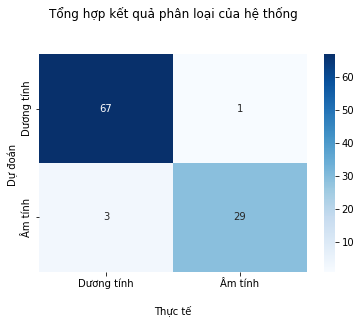
\includegraphics[width=0.66\linewidth]{images/result_backtest}
	\caption{Tổng hợp các ca phân loại của hệ thống.}
	\label{fig:result_backtest}
\end{figure}
Bài toán của luận văn chỉ có hai lớp để phân loại nên phương pháp thích hợp nhất để đánh giá là True/False Positive/Negative. Ta định nghĩa lớp dữ liệu quan trọng hơn cần được xác định đúng là lớp Positive (P-dương tính), lớp còn lại được gọi là Negative (N-âm tính). Ta định nghĩa True Positive (TP), False Positive (FP), True Negative (TN), False Negative (FN) dựa trên confusion matrix chưa chuẩn hoá. 

Bằng phương pháp trên, ta có kết quả tổng hợp tại hình \ref{fig:result_backtest}, tỉ lệ dự đoán chính xác là 96\%, tỉ lệ báo động nhầm (False Alarm Rate) là 1\% và tỉ lệ bỏ sót (Miss Detection Rate) là 3\%.  

	\chapter*{\begin{center}Kết luận\end{center}}
\addcontentsline{toc}{chapter}{Kết luận}
Phân loại ảnh số là một lĩnh vực nghiên cứu hấp dẫn vì có thể áp dụng trong rất nhiều bài toán thực tế. Đây cũng là một bài toán phức tạp nhưng không quá khó để giải quyết nếu ta biết ứng dụng các thành tựu nghiên cứu trong các lĩnh vực như xử lý ảnh số, trí tuệ nhân tạo… Trong đó, việc ứng dụng thành quả của Deep learning mà trong đó đặc biệt là các mô hình của mạng CNN cho ta các kết quả thực sự ấn tượng.

\section*{Kết quả đã đạt được}
Sau một thời gian tìm hiểu nghiên cứu, luận văn đã trình bày được các vấn đề sau:
\begin{itemize}
	\item Trình bày khái quát về CNN và bài toán chẩn đoán bệnh lao
	\item Hệ thống hóa một số mô hình học sâu hỗ trợ chẩn đoán
	\item Cài đặt thử nghiệm một trong các mô hình đã được hệ thống hóa
\end{itemize}

\section*{Hướng hoàn thiện và phát triển tiếp theo:}
Chương trình tuy đã đảm bảo được những chức năng chính yếu nhất của luận văn, nhưng để áp dụng vào thực tế thì vẫn chưa thể được. Lý do chính cho việc này là do sự khác biệt giữa nguồn ảnh đầu vào. Như đã trình bày ở Chương 3, nguồn ảnh đầu vào của bài toán luận văn là ảnh định dạng PNG, tuy nhiên, thực tế nguồn ảnh x-quang y tế được chụp qua các thiết bị thu nhận ảnh y tế (CT, MRI...) hầu hết lại ở định dạng DICOM. Việc không đồng nhất về định dạng ảnh khiến cho chương trình hiện nay chưa thể đưa vào sử dụng trong thực tế.

Một vấn đề khác khi nghiên cứu bài toán của luận văn với bộ dữ liệu do Tawsifur Rahman và cộng sự \cite{dataset} cung cấp là chất lượng ảnh đầu vào không đồng đều. Hầu hết ảnh trong bộ dữ liệu đều có chất lượng tốt, sắc nét, rõ ràng. Nhưng cũng có một vài ảnh mờ, không thực sự rõ nét. Ảnh chất lưởng kém hơn ít nhiều cũng sẽ ảnh hưởng đến độ chính xác của chương trình. Việc nâng cao chất lượng ảnh đầu vào cho chương trình nói riêng và cả lĩnh vực Thị giác Máy - Computer Vision - nói chung là vấn đề rất quan trọng. 

Từ những vấn đề nêu trên, học viên đề xuất hướng phát triển tiếp theo là hoàn thiện thêm các chức năng liên quan đến nâng cao chất lượng ảnh đầu vào, chức năng kết nối với thiết bị thu nhận ảnh y tế (CT, MRI...) để hoàn thiện chương trình có thể ứng dụng vào thực tiễn.
	\addcontentsline{toc}{chapter}{Tài liệu tham khảo}
\begin{thebibliography}{99}
	\bibitem{gtcreport} WHO {\it Global tuberculosis report 2020}, báo cáo tại \href{https://www.who.int/publications/i/item/9789240013131}{ https://www.who.int/publications/i/item/9789240013131}, 2020
	
	\bibitem{bytchuandoanlao} Bộ Y tế {\it Chuẩn đoán bệnh lao}, \href{https://healthvietnam.vn/thu-vien/tai-lieu-tieng-viet/ho-hap/chan-doan-benh-lao}{https://healthvietnam.vn/thu-vien/tai-lieu-tieng-viet/ho-hap/chan-doan-benh-lao}, 2015
	
	%\bibitem{ntt8b3} Nguyễn Thanh Tuấn {\it Neural network}, https://nttuan8.com/bai-3-neural-network, 2019
	
	\bibitem{ntt} Nguyễn Thanh Tuấn {\it Deep learning cơ bản (Chưa xuất bản)}, \href{https://drive.google.com/file/d/1lNjzISABdoc7SRq8tg-xkCRRZRABPCKi/view}{https://drive.google.com/file/d/1lNjzISABdoc7SRq8tg-xkCRRZRABPCKi/view}, 2019
	
	\bibitem{densenetlagi} Võ Thị Một, Võ Duy Nguyên, Nguyễn Tấn Trần Minh Khang {\it Trích chọn đặc trưng và phân loại ảnh x-quang phổi}, TNU Journal of Science and Technology 226(07): 182 - 189 {\href{http://jst.tnu.edu.vn/jst/article/viewFile/3974/pdf}{PDF}}, 2021
	
	\bibitem{dataset} Tawsifur Rahman, Amith Khandakar, Muhammad A. Kadir, Khandaker R. Islam, Khandaker F. Islam, Zaid B. Mahbub, Mohamed Arselene Ayari, Muhammad E. H. Chowdhury {\it Reliable Tuberculosis Detection using Chest X-ray with Deep Learning, Segmentation and Visualization}, IEEE Access - Vol. 8, 2020
	
	\bibitem{cnnhumanbrain} Grace W. Lindsay {\it Convolutional Neural Networks as a Model of the Visual System: Past, Present, and Future}, arXiv - Cornell University (\href{https://arxiv.org/ftp/arxiv/papers/2001/2001.07092.pdf}{PDF}), 2001
	
	\bibitem{vgg16} Karen Simonyan, Andrew Zisserman {\it Very deep convolutional networks for large-scale image recognition}, ICLR 2015 (\href{https://arxiv.org/pdf/1409.1556.pdf}{PDF}), 2015
	
	\bibitem{densenet} Gao Huang, Zhuang Liu, Laurens van der Maaten, Kilian Q. Weinberger {\it Densely Connected Convolutional Networks}, arXiv:1608.06993 (\href{https://arxiv.org/pdf/1608.06993.pdf}{PDF}), 2016 
	  
\end{thebibliography}

	
\end{document}


